\documentclass[a4paper]{article}

\usepackage[table]{xcolor}%this has to be the first!!!!!!
\usepackage{fullpage} % Package to use full page
%\usepackage{parskip} % Package to tweak paragraph skipping
\usepackage{tikz} % Package for drawing
\usetikzlibrary{shapes,arrows,matrix,positioning}
\usepackage{amsmath}
\usepackage{indentfirst}
\usepackage{hyperref}
\usepackage{subcaption}
\usepackage{graphics}
\usepackage{graphicx}
\usepackage{minted}
\usepackage{multicol}
\usepackage{mathrsfs}
%color define
\definecolor{codebg}{RGB}{230,255,253}
\definecolor{function}{RGB}{210,0,26}
\definecolor{para}{RGB}{255,137,137}
\definecolor{output}{RGB}{238,224,201}
\setminted[cpp]{mathescape=true,breaklines,bgcolor=codebg,linenos}

\tikzset{
  block/.style = {rectangle, draw, fill=output, text width=6cm, text centered, rounded corners, minimum height=4em},
  line/.style = {draw, -latex'},
}

%function newcommand
\newcommand{\func}[1]{\textbf{\textcolor{function}{#1}}}
\newcommand{\para}[1]{\textbf{\emph{\textcolor{para}{#1}}}}

%other examples for icon in text
%WARNING: the number is not allowed in newcommand name
\newcommand{\testA}{\tikz \fill[brown] (2pt,2pt) rectangle (8pt,8pt);}
\newcommand{\testB}{\tikz \fill[black] (3pt,3pt) circle (3pt);}

\usepackage{biblatex}
\addbibresource{bibliography.bib}
\title{embed-tree.h documentation}
\author{Haochen(Langford) Huang}
\date{\today}

\makeatletter%title setting
\def\@maketitle{%
  \newpage
  \null
  \vskip 2em%
  \begin{center}%
  \let \footnote \thanks
    {\LARGE \@title \par}%
    \vskip 1.5em%
    {\Large
      \lineskip .5em%
      \begin{tabular}[t]{c}%
        \@author
      \end{tabular}\par}%
    \vskip 1em%
    {\large \@date\par}%
    \vskip 1em%
    {\large version:draft}%
  \end{center}%
  \par
  \vskip 1.5em}
\makeatother

\begin{document}

\maketitle
\section{Introduction}
Current header file provides restriction, prolongation and refinement under tree grid for corresponding value employed in \textbf{embed.h}. The content can be separated into two parts: the refinement of cut-cell value i.e. \para{cs} and \para{fs} and the restriction/prolongation of value on cut-cell and cut-face.

\section{Refinement of Embed associated value}
\subsection{\func{embed\_fraction\_refine}}
\func{embed\_fraction\_refine} calculates the volume fraction contained by each child cell.
\subsubsection{Worth Mentioning Details}
\begin{figure}[h]
    \centering
    \begin{subfigure}[b]{0.45\textwidth}
        \centering
        \includegraphics[height=6cm]{image/fraction_refine2D1.pdf}
        \subcaption{}
        \label{fig:2Drefine1}
    \end{subfigure}
    \begin{subfigure}[b]{0.45\textwidth}
        \centering
        \includegraphics[height=6cm]{image/fraction_refine2D2.pdf}
        \subcaption{}
        \label{fig:2Drefine2}
    \end{subfigure}
    \caption{Refinement of embed fraction \para{cs}. By switching the component of normal direction $\mathbf{n}$, the program rotates the interface therefore iterating volume fraction of each subcell.}
    \label{fig:2Drefine}
\end{figure}
For cells contains interface, 
given the function \func{rectangle\_fraction} from \textbf{geometry.h} as well as interface information $\mathbf{n},\alpha$, the volume fraction inside child cell can be obtained. Figure \ref{fig:2Drefine1} depicts an example under $2D$ condition in which the area inside child cell highlighted by red dashed is calculated.\par
In stead of switching the computational domain (i.e. the red dashed cell), the program achieve iteration between cells by switching the sign of normal direction as indicated by figure \ref{fig:2Drefine2}.

\subsubsection{Parameters}
\hfill
\begin{table}[h]
  \centering
  \begin{tabular}{|c|c|c|c|c|}
    \hline
    Name & Data type & Status & Option & Representation (before/after)\\[0.5ex]
    \hline\hline
    \para{point} & Point & unchanged & compulsory & position index\\
    \hline
    \para{cs} & scalar & unchanged & compulsory & volume fraction $cs$\\
    \hline
  \end{tabular}
\end{table}

\subsubsection{Program Workflow}
\vspace{1mm}
\begin{multicols}{2}
  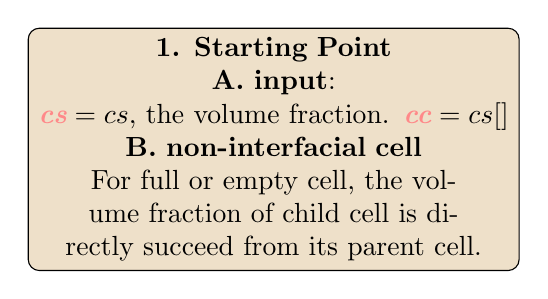
\begin{tikzpicture}
    \node [block](init){
        \textbf{1. Starting Point}\\
        \textbf{A. input}: \\
        $\para{cs}=cs$, the volume fraction.
        $\para{cc}=cs[]$\\
        \textbf{B. non-interfacial cell}\\
        For full or empty cell, the volume fraction of child cell is directly succeed from its parent cell.
      };
  \end{tikzpicture}
 \columnbreak
 \begin{minted}{cpp}
static void embed_fraction_refine (Point point, scalar cs)
{
  double cc = cs[];
  if (cc <= 0. || cc >= 1.) {
    foreach_child()
      cs[] = cc;
  }
 \end{minted}
\end{multicols}

\begin{center}
  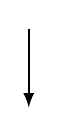
\begin{tikzpicture}
    \draw[-latex,thick](0,0) -- (0,-1); 
  \end{tikzpicture}
\end{center}

\begin{multicols}{2}
  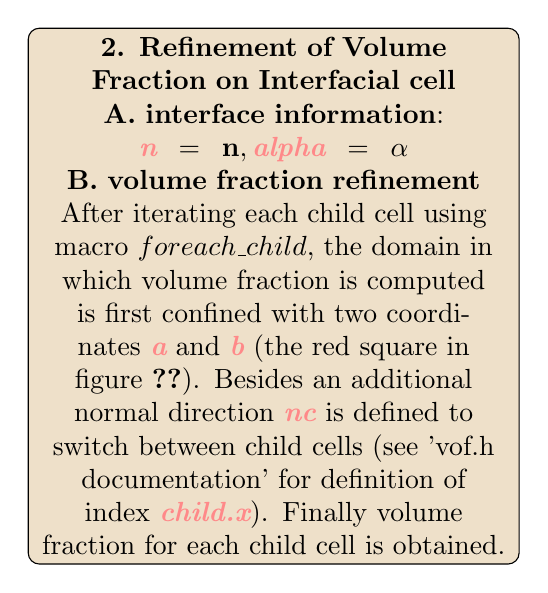
\begin{tikzpicture}
    \node [block](init){
        \textbf{2. Refinement of Volume Fraction on Interfacial cell}\\
        \textbf{A. interface information}: \\
        $\para{n}=\mathbf{n},\para{alpha}=\alpha$\\
        \textbf{B. volume fraction refinement}\\
        After iterating each child cell using macro $foreach\_child$, the domain in which volume fraction is computed is first confined with two coordinates \para{a} and \para{b} (the red square in figure \ref{fig:2Drefine}). Besides an additional normal direction \para{nc} is defined to switch between child cells (see 'vof.h documentation' for definition of index \para{child.x}). Finally volume fraction for each child cell is obtained.
      };
  \end{tikzpicture}
 \columnbreak
 \begin{minted}{cpp}
    coord n = facet_normal (point, cs, fs);
    double alpha = plane_alpha (cc, n);
      
    foreach_child() {
      static const coord a = {0.,0.,0.}, b = {.5,.5,.5};
      coord nc;
      foreach_dimension()
	nc.x = child.x*n.x;
      cs[] = rectangle_fraction (nc, alpha, a, b);
    }
  }
}
 \end{minted}
\end{multicols}

\subsection{\func{embed\_face\_fraction\_refine}}
Given face vector \para{fs} on mesh level $N$, function \func{embed\_face\_fraction\_refine} returns \para{fs} on finer mesh level $N+1$. Computation of face fraction is achieved by first computing the fraction of 'inner' faces then the 'boundary' faces both under $2D$ and $3D$ conditions. For sake of convenience, the implementation on $2D$ cases is first introduced then followed by the implementation on $3D$ condition. The program however is arranged based on computation on 'inner' faces or 'boundary' faces.\par
Note that the function is duplicated by macro $foreach\_dimension$ and each function is only responsible for facial fraction computation on one direction. The introduction shall take computation on $x$ as an example hereinafter.\par
Moreover, for a cut-cell ($\para{cs} \in (0,1)$) the interface exclusively yields as 
\begin{equation}\label{equ:interface}
    \mathbf{n}\cdot\mathbf{x} = \alpha
\end{equation}
where $\mathbf{n}$ is the normal direction of the interface, $\mathbf{x}$ represents coordinates of arbitrary point at the interface and $\alpha$ is the constant. This holds true for both condition and is the critical in identifying different condition in the upcoming sections.
\subsubsection{$2D$ Condition}
First consider the fine faces contained inside the cell as shown by $A,B$ in figure \ref{fig:2Dinner}.\par
\begin{figure}[h]
    \centering
    \includegraphics[height=6cm]{image/fs_2D.pdf}
    \caption{Sketch for inner fine faces $A,B$, two red lines display example threshold value for the interfaces.}
    \label{fig:2Dinner}
\end{figure}
The very first step to compute face fraction is to identify whether the interface comes across the inner fine faces. Given $\alpha=\alpha_1$ and $\mathbf{n}=(n_x,n_y)$ of the interface and coordinate system whose $(0,0)$ locates at center of the cell, the lower and upper boundary for the condition is the line set passing $(0,0.5),(0,-0.5)$ respectively. According to equation \ref{equ:interface}, once
\begin{equation}\label{equ:judge}
    |2\alpha_1|<|n_y|
\end{equation}
the interface will come across the inner fine faces otherwise both the face fraction are $0$ or $1$ determined by interface direction.
If equation \ref{equ:judge} holds true the intersection point $(0,y_i)$ between interface and y-axis yields $y_i = \frac{\alpha}{n_y}$. The face fraction for face $A,B$ therefore can be obtained accordingly.\par
\begin{figure}[h]
    \centering
    \includegraphics[height=6cm]{image/fs_2D2.pdf}
    \caption{Sketch for boundary fine faces $C,D$, the numerical labels mark the corresponding transverse faces.}
    \label{fig:2Dboundary}
\end{figure}
Following a similar process, the boundary fine face fraction is calculated first by identifying the intersection point (if exists) then computing the fine face fraction. Different from the previous, the face fraction can be visited directly without equation \ref{equ:judge}. The orientation of the interface is obtained by checking corresponding transverse faces as shown by (1-4) in figure \ref{fig:2Dboundary}. Combined with face fraction on original face, the fine face fraction is therefore obtained.

\subsubsection{$3D$ Condition}
\begin{figure}[h]
    \centering
    \begin{subfigure}[b]{0.45\textwidth}
        \centering
        \includegraphics[height=6cm]{image/fs_3D3.pdf}
        \subcaption{}
        \label{fig:3Dinner}
    \end{subfigure}
    \begin{subfigure}[b]{0.45\textwidth}
        \centering
        \includegraphics[height=6cm]{image/fs_3D4.pdf}
        \subcaption{}
        \label{fig:3Dboundary}
    \end{subfigure}
    \caption{Inner fine face (a) and boundary fine face (b) under 3D condition. The red contour highlights the cell where projection takes place.}
    \label{fig:3Dface}
\end{figure}
\begin{figure}[hp]
    \centering
    \begin{subfigure}[b]{0.45\textwidth}
        \centering
        \includegraphics[height=6cm]{image/fs_3D1.pdf}
        \subcaption{}
        \label{fig:3Dinner1}
    \end{subfigure}
    \begin{subfigure}[b]{0.45\textwidth}
        \centering
        \includegraphics[height=6cm]{image/fs_3D2.pdf}
        \subcaption{}
        \label{fig:3Dinner2}
    \end{subfigure}

    \begin{subfigure}[b]{0.45\textwidth}
        \centering
        \includegraphics[height=6cm]{image/fs_3D5.pdf}
        \subcaption{}
        \label{fig:3Dinner3}
    \end{subfigure}
    \caption{A zoom in for highlighted cell in figure \ref{fig:3Dface}. (a) The original interface and (b) the projection interface for inner face in figure \ref{fig:3Dinner} and (c) the original interface for boundary fine face in figure \ref{fig:3Dboundary}.}
\end{figure}
The fine face fraction for both inner and boundary faces are computed directly using $2D$ projection from a $3D$ interface.\par

First consider the inner face, as shown by figure \ref{fig:3Dinner}, the fine face fraction is computed from $2D$ projection in red contour cell. Moreover the iteration is accomplished among four subcells by rotating the whole interface as in section (unfinished). Specifically, 
given $\mathbf{n}=(n_x,n_y,n_z)$ and $\alpha=\alpha_1$ of the example interface shown by figure \ref{fig:3Dinner1}, the face fraction on the inner fine face can be obtained by calculating the volume fraction of reconstructed interface shown by figure \ref{fig:3Dinner2}. Since the volume calculation can be achieved by tool provided by \textbf{geometry.h}, the problem degenerates as how to reconstruct the interface and get its $\mathbf{n},\alpha$.\par

Note the fact that the reconstructed interface is perpendicular to the projection plane and comes across the same line as original interface on projection plane, its $\mathbf{n}=(0,n_y,n_z), \alpha=\alpha_1$.\par

Similarly, the fine face fraction on boundary face is also computed by projection but on the boundary plane. An example is shown by figure \ref{fig:3Dinner3} where reconstructed plane should pass the intersection line on boundary face (blue line) as well as the red dashed. Given an arbitrary point set $(0.5,y_1,z_1),(0,y_1,z_1)$ the $\alpha=\alpha_2$ of the reconstructed interface has relation:
\begin{align}
    0.5n_x+y_1n_y+z_1n_z &= \alpha_1\\
    y_1n_y+z_1n_z &= \alpha_2\\
    \alpha_2 &= \alpha_1-0.5n_x\label{equ:alphabf}
\end{align}
Consider the normal direction $(0,n_y,n_z)$, the face fraction therefore can be calculated.
\newpage
\subsubsection{Worth Mentioning Details}
\begin{figure}[hp]
    \centering
    \includegraphics[height=6cm]{image/fine.pdf}
    \caption{Index for \func{fine}.}
    \label{fig:finefunc}
\end{figure}
Apart from geometric formula, function \func{fine} is called multiple times to visit data on finer mesh. The index for facce vector of subcell is demonstrated in figure \ref{fig:finefunc} which can be directly deduced into $3D$ condition.


\subsubsection{Parameters}
\hfill
\begin{table}[h]
  \centering
  \begin{tabular}{|c|c|c|c|c|}
    \hline
    Name & Data type & Status & Option & Representation (before/after)\\[0.5ex]
    \hline\hline
    \para{point} & Point & unchanged & compulsory & position index\\
    \hline
    \para{s} & scalar & unchanged & compulsory & volume fraction $cs$\\
    \hline
  \end{tabular}
\end{table}

\subsubsection{Program Workflow}
\begin{multicols}{2}
  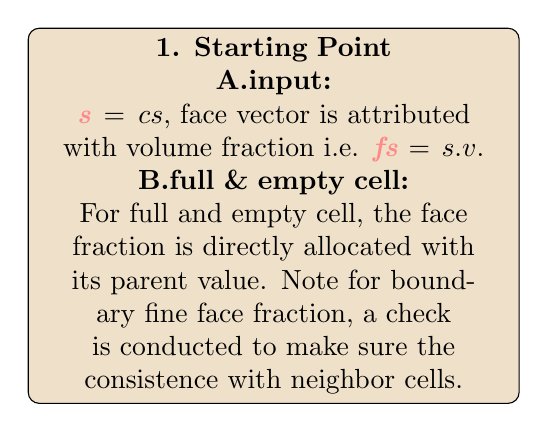
\begin{tikzpicture}
    \node [block]{
        \textbf{1. Starting Point}\\
        \textbf{A.input:} \\
        $\para{s} = cs$,
        face vector is attributed with volume fraction i.e. $\para{fs}=s.v$.\\
        \textbf{B.full \& empty cell:}\\
        For full and empty cell, the face fraction is directly allocated with its parent value. Note for boundary fine face fraction, a check is conducted to make sure the consistence with neighbor cells.
      };
  \end{tikzpicture}
 \columnbreak
 \begin{minted}{cpp}
foreach_dimension()
static void embed_face_fraction_refine_x (Point point, scalar s)
{
  vector fs = s.v;
  if (cs[] <= 0. || cs[] >= 1.) {
    for (int j = 0; j <= 1; j++)
      for (int k = 0; k <= 1; k++)
	fine(fs.x,1,j,k) = cs[];
    for (int i = 0; i <= 1; i++)
      if (!is_refined(neighbor(2*i-1)) && neighbor(2*i-1).neighbors &&
	  (is_local(cell) || is_local(neighbor(2*i-1))))
	for (int j = 0; j <= 1; j++)
	  for (int k = 0; k <= 1; k++)
	    fine(fs.x,2*i,j,k) = fs.x[i];
  }
 \end{minted}
\end{multicols}

\begin{center}
  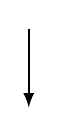
\begin{tikzpicture}
    \draw[-latex,thick](0,0) -- (0,-1); 
  \end{tikzpicture}
\end{center}

\begin{multicols}{2}
  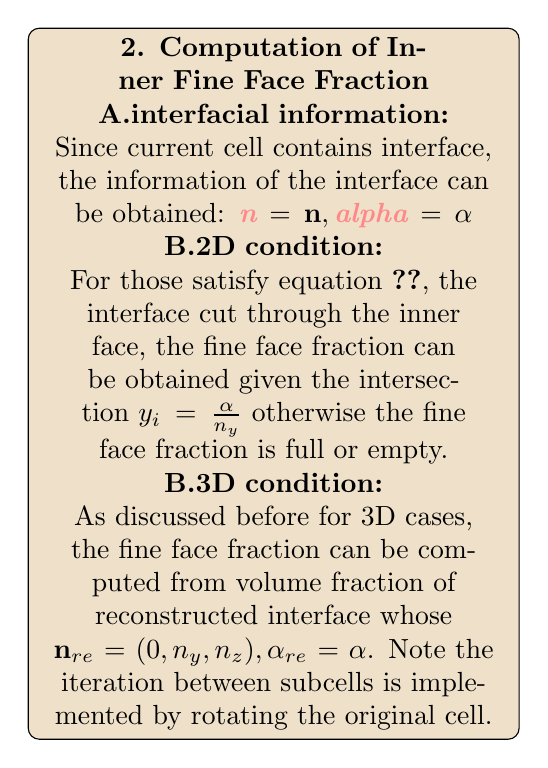
\begin{tikzpicture}
    \node [block]{
        \textbf{2. Computation of Inner Fine Face Fraction}\\
        \textbf{A.interfacial information:} \\        
        Since current cell contains interface, the information of the interface can be obtained: $\para{n}=\mathbf{n},\para{alpha}=\alpha$\\
        \textbf{B.2D condition:} \\
        For those satisfy equation \ref{equ:judge}, the interface cut through the inner face, the fine face fraction can be obtained given the intersection $y_i=\frac{\alpha}{n_y}$ otherwise the fine face fraction is full or empty.\\
        \textbf{B.3D condition:}\\
        As discussed before for 3D cases, the fine face fraction can be computed from volume fraction of reconstructed interface whose $\mathbf{n}_{re} = (0,n_y,n_z), \alpha_{re} = \alpha$. Note the iteration between subcells is implemented by rotating the original cell.
      };
  \end{tikzpicture}
 \columnbreak
 \begin{minted}{cpp}
  else {
    coord n = facet_normal (point, cs, fs);
    double alpha = plane_alpha (cs[], n);
#if dimension == 2
    if (2.*fabs(alpha) < fabs(n.y)) {
      double yc = alpha/n.y;
      int i = yc > 0.;
      fine(fs.x,1,1 - i) = n.y < 0. ? 1. - i : i;
      fine(fs.x,1,i) = n.y < 0. ? i - 2.*yc : 1. - i + 2.*yc;
    }
    else
      fine(fs.x,1,0) = fine(fs.x,1,1) = alpha > 0.;

#else // dimension == 3
    for (int j = 0; j <= 1; j++)
      for (int k = 0; k <= 1; k++)
	if (!fine(cs,0,j,k) || !fine(cs,1,j,k))
	  fine(fs.x,1,j,k) = 0.;
	else {
	  static const coord a = {0.,0.,0.}, b = {.5,.5,.5};
	  coord nc;
	  nc.x = 0., nc.y = (2.*j - 1.)*n.y, nc.z = (2.*k - 1.)*n.z;
	  fine(fs.x,1,j,k) = rectangle_fraction (nc, alpha, a, b);
	}

#endif // dimension == 3
 \end{minted}
\end{multicols}

\begin{center}
  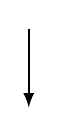
\begin{tikzpicture}
    \draw[-latex,thick](0,0) -- (0,-1); 
  \end{tikzpicture}
\end{center}
\newpage

\begin{multicols}{2}
  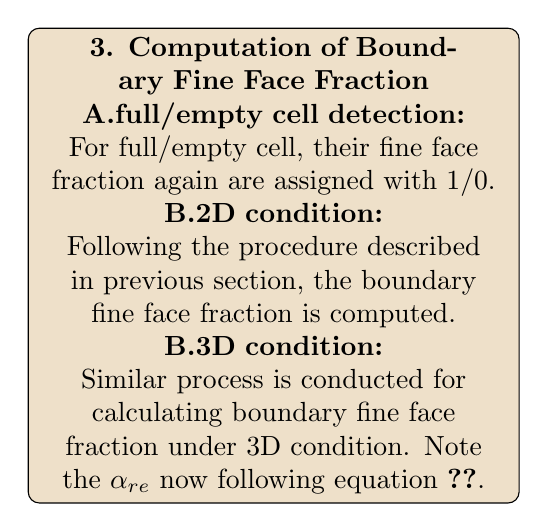
\begin{tikzpicture}
    \node [block]{
        \textbf{3. Computation of Boundary Fine Face Fraction}\\
        \textbf{A.full/empty cell detection:} \\
        For full/empty cell, their fine face fraction again are assigned with $1/0$.\\
        \textbf{B.2D condition:} \\
        Following the procedure described in previous section, the boundary fine face fraction is computed.\\
        \textbf{B.3D condition:}\\
        Similar process is conducted for calculating boundary fine face fraction under 3D condition. Note the $\alpha_{re}$ now following equation \ref{equ:alphabf}.
      };
  \end{tikzpicture}
 \columnbreak
 \begin{minted}{cpp}
    for (int i = 0; i <= 1; i++)
      if (neighbor(2*i-1).neighbors &&
	  (is_local(cell) || is_local(neighbor(2*i-1)))) {
	if (!is_refined(neighbor(2*i-1))) {
	  if (fs.x[i] <= 0. || fs.x[i] >= 1.)
	    for (int j = 0; j <= 1; j++)
	      for (int k = 0; k <= 1; k++)
		fine(fs.x,2*i,j,k) = fs.x[i];
	  else {
#if dimension == 2
	    double a = fs.y[0,1] <= 0. || fs.y[2*i-1,1] <= 0. ||
	      fs.y[] >= 1. || fs.y[2*i-1] >= 1.;
	    if ((2.*a - 1)*(fs.x[i] - 0.5) > 0.) {
	      fine(fs.x,2*i,0) = a;
	      fine(fs.x,2*i,1) = 2.*fs.x[i] - a;
	    }
	    else {
	      fine(fs.x,2*i,0) = 2.*fs.x[i] + a - 1.;
	      fine(fs.x,2*i,1) = 1. - a;
	    }

#else  // dimension == 3
	    for (int j = 0; j <= 1; j++)
	      for (int k = 0; k <= 1; k++) {
		static const coord a = {0.,0.,0.}, b = {.5,.5,.5};
		coord nc;
		nc.x = 0., nc.y = (2.*j - 1.)*n.y, nc.z = (2.*k - 1.)*n.z;
		fine(fs.x,2*i,j,k) =
		  rectangle_fraction (nc, alpha - n.x*(2.*i - 1.)/2., a, b);
	      }

#endif // dimension == 3
	  }
	}
 \end{minted}
\end{multicols}

\begin{center}
  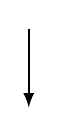
\begin{tikzpicture}
    \draw[-latex,thick](0,0) -- (0,-1); 
  \end{tikzpicture}
\end{center}

\begin{multicols}{2}
  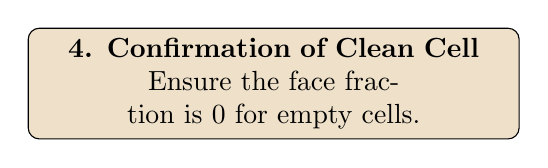
\begin{tikzpicture}
    \node [block]{
        \textbf{4. Confirmation of Clean Cell}\\
        Ensure the face fraction is $0$ for empty cells.
      };
  \end{tikzpicture}
 \columnbreak
 \begin{minted}{cpp}
	for (int j = 0; j <= 1; j++)
	#if dimension > 2
	  for (int k = 0; k <= 1; k++)
	#endif
	    if (fine(fs.x,2*i,j,k) && !fine(cs,i,j,k))
	      fine(fs.x,2*i,j,k) = 0.;
      }
  }
}
 \end{minted}
\end{multicols}

\section{Readme}
Normally, a documentation would consist of two major parts: Introduction \& Backround and Function. The first part will introduce the purpose of the corresponding program and the governing equations it solved and other thing developers and users should be aware of \emph{e.g.} in which method the program solve the overall problem. Pragmatic program will be explored line by line in the second part. It first contains a table to clearify all the parameters and their physical representatives as shown in Table.\ref{tab:test}. 
\begin{table}[h]
  \centering
  \begin{tabular}{|c|c|c|c|c|}
    \hline
    Name & Data type & Status & Option & Representation (before/after)\\[0.5ex]
    \hline\hline
    \rowcolor{output} \para{a} & scalar* & update & complusory & $\delta \mathbf{u}^{*,k}/\delta \mathbf{u}^{*,k+1}$\\
    \hline
    \para{b} & scalar* & unchange & complusory & $RES$\\
    \hline
    \para{dt} & double & unchange & complusory & $\Delta t$\\
    \hline
    \para{l} & int & unchange & complusory &  mesh level \\
    \hline
    \para{data} & struct Vsicosity & unchange & complusory & $\mu^ {n+\frac{1}{2}}, \rho^{n+\frac{1}{2}}, \Delta t$ \\
    \hline
  \end{tabular}
  \caption{Referenc table of parameters.}
  \label{tab:test}
\end{table}
The highlighted row in the table indicates such paramter is either the output or has been updated. Second subsection always concerns with detals and specific technique the function employed. Finally the third part is the workflow of the program.\par
Throughout documentation font \para{para} represents exact name of parameters and \func{function} represents exact name of the function.

Tikz inside text example: $\testA$.

\section{Program Workflow Example}
\vspace{1mm}
\begin{multicols}{2}
  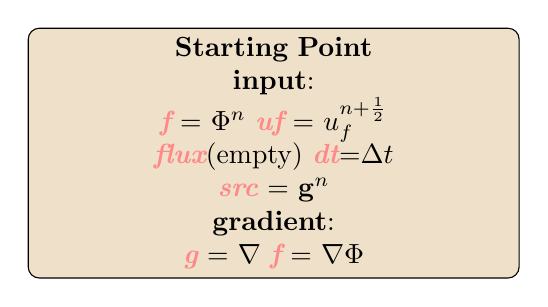
\begin{tikzpicture}
    \node [block](init){
        \textbf{Starting Point}\\
        \textbf{input}: \\
        \para{f} = $\Phi^n$ \para{uf} = $u_f^{n+ \frac{1}{2}}$\\ \para{flux}(empty) \para{dt}=$\Delta t$\\ \para{src} = $ \mathbf{g}^n$\\
        \textbf{gradient}:\\
        \para{g} = $\nabla$ \para{f} = $\nabla \Phi$
      };
  \end{tikzpicture}
 \columnbreak
 \begin{minted}{cpp}
void tracer_fluxes (scalar f,
		    face vector uf,
		    face vector flux,
		    double dt,
		    (const) scalar src)
{
  vector g[];
  gradients ({f}, {g});
 \end{minted}
\end{multicols}

\begin{center}
  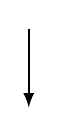
\begin{tikzpicture}
    \draw[-latex,thick](0,0) -- (0,-1); 
  \end{tikzpicture}
\end{center}

\printbibliography
\end{document}
